
\documentclass[conference]{IEEEtran}


\usepackage[letterpaper, left=1.01in, right=1.01in, bottom=1in, top=0.75in]{geometry}

\usepackage{setspace}
\usepackage{mathrsfs}
\usepackage{amsmath}
\usepackage{amsfonts}
\usepackage{amsthm}
\usepackage{amssymb}
\usepackage{graphicx}
\usepackage{subfigure}
\usepackage{indentfirst}
\usepackage{array}
\usepackage{cite}
\usepackage{enumerate}
\usepackage{multirow}
\usepackage{verbatim}
\usepackage{stfloats}
\usepackage{color}

\begin{document}

\title{Sparsely Connected Neural Network for Massive MIMO Detection}

\author{\IEEEauthorblockN{Guili Gao$^{1,2}$, Chao Dong$^{1,2}$, Kai Niu$^1$}
\IEEEauthorblockA{
$^{1}$Key Laboratory of Universal Wireless Communications, Ministry of Education\\
Beijing University of Posts and Telecommunications \\
$^{2}$Science and Technology on Communication Networks Laboratory\\
Email: \{2016140061, dongchao, niukai\}@bupt.edu.cn}
}

% make the title area
\maketitle

% As a general rule, do not put math, special symbols or citations
% in the abstract
\begin{abstract}
Deeping learning can achieve high parallelism and robustness, which is especially suitable for massive multiple-input multiple-output (MIMO) detection. There are already some well-developed deep learning models applied to MIMO detection, in which detection network is a typical representative model with excellent performance, but its complexity is high. This paper aims to simplify the detection network model, and the simplification runs through the entire data processing. This simplification includes three improvements. First, the number of inputs is reduced to simplify inputs; Second, the network connection structure is simplified by changing network from full connectivity to sparsely connectivity and reducing the number of network layers by half. Third, the loss function optimizes to avoid irreversible problems with the matrix. Base on the above improvements, the complexity of the network is reduced from ${\mathcal{O}(64n^2)}$ to ${\mathcal{O}(3n)}$. The simulation results indicates that the proposed structure has better performance than the existing detection network.
\end{abstract}

\IEEEpeerreviewmaketitle



\section{Introduction}
% no \IEEEPARstart
Multiple-input multiple-output (MIMO) technology can improve spectrum efficiency and has been applied in many wireless communication standards, such as WiMax and LTE \cite{LTE}\cite{MIMO1}. Basically, the more antennas the transmitter/receiver is equipped with, the more possible signal paths and the better the performance in terms of data rate and link reliability. In future 5G development, massive MIMO is considered as a key technique with number of transmission and receiving antennas. It is getting great attention for need of high communication data rate, however, most of the MIMO used today is ${4 \times 4}$ or ${8 \times 8}$. One of the reasons is that with the number of antennas increase, the complexity becomes large, which is one of the key factors that restrict the number of antennas. So the key issue in using the massive MIMO is to reduce the detection complexity. The optimal detection scheme is the maximum likelihood (ML) detection, but it has the highest computational complexity. To reduce computational complexity, the linear detector is proposed, such as the minimum mean squared error (MMSE) and zero-forcing (ZF)\cite{MIMO2} detectors. But the performance of linear detection is poor. There are other suboptimal algorithms, including approximate message passing (AMP)\cite{AMP}, semidefinite relaxation (SDR)\cite{SDR}, \cite{detector} and fixed-complexity sphere decoder (FSD)\cite{FSD}. There are many simplifying algorithms, but as the number of antennas increases, their complexity becomes intolerable and performance deteriorates.

In the past few years, machine learning has achieved a great success in many fields. There are many models in the field of machine learning, such as Support Vector Machine (SVM), XGBoost\cite{XGBoost}, Decision Tree and Neural Networks. The rapidest development in recent years is the deep learning, especially in image processing and artificial intelligence. Deep learning is a multi-layer neural network constructed by complex connections, and the network structure is adjusted according to different application scenarios. The use of neural networks consists of two phases, training phase and application phase. During the training phase, pre-marked data are inputed into the network to adjust the network connection weights. The most commonly used network weight adjustment algorithm is the gradient descent method. But with the increase of network layer, the training time will increase, and the gradient will radiate or disappear\cite{normalization}. Residual neural network (ResNet)\cite{ResNet} can increase the depth of the network, speed up convergence, improve the performance of the network, and avoid problems such as the radiation or the disappearing caused by too much network layer. ResNet is referenced in the network structure of this paper.

Detection network (DetNet)\cite{DetNet} is a multilayer deep neural network for massive MIMO detection. The performance of DetNet is much better than that of MMSE and ZF, especially when the number of antennas increases, it can approach the performance of AMP algorithm. The process of DetNet contains two phases. the training phase and the detection phase. During training, base on the number of antennas and receiving antennas, and the number of nodes in the network is determined; Each batch of training data run though different fast fading channels and different signal-to-noise ratio (SNR). The receiver will input the receiving signals into the network for training. The convergence of training parameters is guaranteed by backward propagation algorithm. In detection phase, the network has been trained, the weights of network are fixed, and they can be applied to different fast fading channels and different SNRs. The following are the advantages and disadvantages of DetNet.
\begin{itemize}
\item Advantage:
    \begin{enumerate}
        \item  The performance of DetNet is similar to the performance of suboptimal algorithm, and with the increase of the number of antennas, the performance is better.
        \item  DetNet has good robustness, once trained, they can adapt to different SNR and different channels.
        \item  The structure of DetNet can be processed in parallel, especially when the current computing chip is providing better support for the parallel computing.
    \end{enumerate}
\item Disadvantages:
    \begin{enumerate}
        \item  When the number of antennas is small, the performance is worse than linear detection.
        \item  DetNet requires that the transmitter has fewer sending antennas than the receiving end, and if the number of sending antennas is close to or larger than the number of receiving antennas, the performance will be poor.
    \end{enumerate}
\end{itemize}

%The use of deep learning to solve the problem of wireless communication is an inevitable transition from wireless communication to intelligent communication, and it is also an exploration of solving modern communication problems. We hope to contribute to the progress of future communications.

In this paper, we define the channel matrix as \textbf{H}, the transmit vector as \textbf{x}, and the receive vector as \textbf{y}, Boldface uppercase letters denote matrices, Boldface lowercase letters denote vectors, the superscript ${(\centerdot)^T}$ denotes the transpose.


\section{System Model}
In this section, we first introduce the traditional MIMO detection algorithm, then explain the design idea of the DetNet, and finally introduce the parameters of the DetNet network in detail.

\subsection{MIMO Detection}

For a MIMO system, we consider an end-to-end communication system which contains ${n}$ transmit antennas, ${m}$ receiving antennas, where ${n \textless m}$. The real part is considered, and the imaginary part is ignored. The communication model can be described as follows:

\begin{equation}
\label{basic model}
\textbf{y}=\textbf{Hx}+\textbf{n}
\end{equation}

Where \textbf{y} is a real vector of ${m \times 1}$ dimensions, \textbf{x} is a real vector of ${n \times 1}$ dimensions, \textbf{n} is a real vector of ${m \times 1}$ dimensions representing the additive white gaussian noise (AWGN) of with independent and identically distributed (i.i.d.), each with zero-mean and variance ${{\delta}^2}$, \textbf{H} is ${m \times n}$ matrix, which represents the channel state information (CSI) that is supposed known perfectly.

The goal of MIMO detection is to detecte the transmission signals according to the signals received by the receiving antennas. The best algorithm is ML detection. According to ML, all possible transmission siginals are sent over the known channel, and the detection result is the transmission signals with the output signals which is nearest to receiving siginals based on Euclidean distance. Because ML searches all the possible signals, the complexity of ML detection increases exponentially as the number of antennas and the modulation order increase. This is impractical for massive MIMO detection and the reason why the ML detection is rarely used in practical MIMO detection. The formula (\ref{ML}) is the procedure of ML detection.

\begin{equation}
\label{ML}
\hat{\textbf{x}}=\mathop{\arg\min}_{x\in\{\pm1\}^K}\|\textbf{y-Hx}\|^2
\end{equation}

Although ML detection is hard to be realized in the project, it has an enlightening effect on other detection algorithms. Many  algorithms are derived from ML, DetNet is one of them.

\subsection{DetNet}
DetNet was proposed in "Deep MIMO detection", it is a multi-layer neural network dedicated to MIMO detection, the overall structure of the network is as Fig.\ref{Network model}.

\begin{figure}[ht]
  \centering
  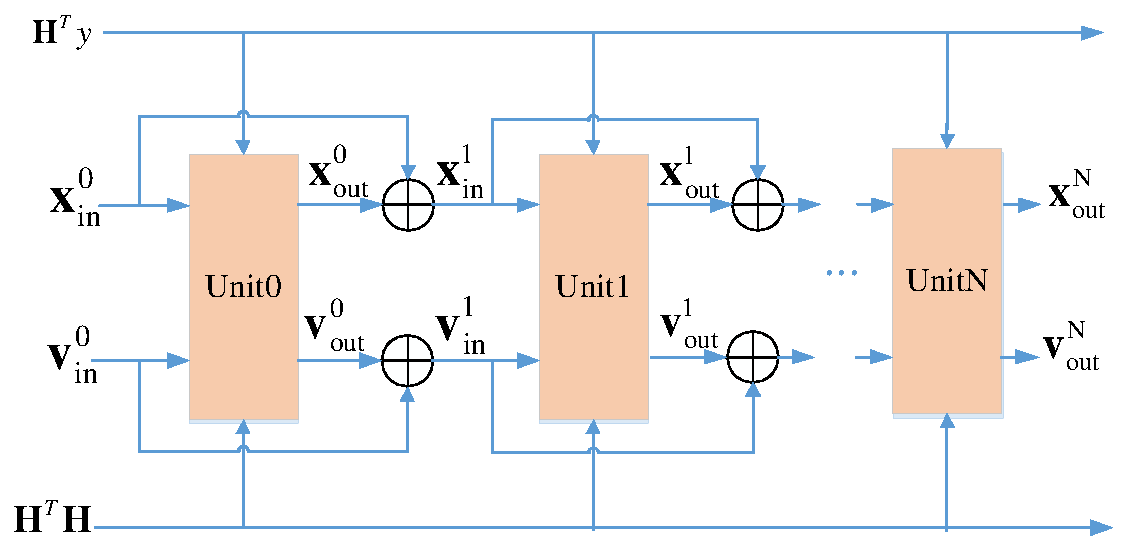
\includegraphics[width=0.45\textwidth]{DetNetFormWork.pdf}
  \caption{DetNet Formwork}
  \label{Network model}
\end{figure}

DetNet is cascaded through multiple units with same structure. There are four inputs in each unit: ${\textbf{H}^T\textbf{y}}$, ${\textbf{H}^T\textbf{H}}$, ${\textbf{x}_{\textrm{in}}^l}$ and ${\textbf{v}_{\textrm{in}}^l}$, where ${\textbf{H}^T\textbf{y}}$ and ${\textbf{H}^T\textbf{H}}$ are the common inputs, ${\textbf{x}_{\textrm{in}}^l}$ and ${\textbf{v}_{\textrm{in}}^l}$ are changes with unit index, $l$ represents the unit index. The residual structure is applied to increase the number of layer, the structure is as the formula (\ref{ResNet}). The input to the unit $l$ is obtained by weighted averaging of the input of unit $l-1$ and output of unit $l-1$.

\begin{equation}
\label{ResNet}
\begin{split}
&{\textbf{x}_{\textrm{in}}^l}=\mu{\textbf{x}_{\textrm{out}}^{l-1}}+(1-\mu)\textbf{x}_{\textrm{in}}^{l-1}\\
&{\textbf{v}_{\textrm{in}}^l}=\mu{\textbf{v}_{\textrm{out}}^{l-1}}+(1-\mu)\textbf{v}_{\textrm{in}}^{l-1}
\end{split}
\end{equation}

$\mu$ is a residual coefficient. DetNet is an iterative network, the output of each unit can be used as the output of the whole network, and as the increasing number of network units, the output of each unit becomes closer to transmittion signals based on Euclidean distance. For better performance, we should make the network as deep as possible. The design idea of the network comes from the formula (\ref{DetNetTheory}).

\begin{equation}
\label{DetNetTheory}
\begin{split}
\textbf{x}_{\textrm{in}}^{l+1} &=\prod\left[\textbf{x}_{\textrm{in}}^{l}-\lambda_l\left.\frac{\partial\|\textbf{y}-\textbf{Hx}\|^2}{\partial\textbf{x}}\right|_{\textbf{x}=\textbf{x}_{\textrm{in}}^l}\right]\\
&=\prod\left[\textbf{x}_{\textrm{in}}^l-2\lambda_l\textbf{H}^T\textbf{y}+2\lambda_l\textbf{H}^T\textbf{Hx}^l_{\textrm{in}}\right]
\end{split}
\end{equation}

${\textbf{x}_{\textrm{in}}^l}$ is the estimated signal of unit ${l-1}$ and $\lambda_l$ is the stepping parameter. ${\prod}$ is a interative structure. ${\textrm{x}}$ init with a random vector, as the structure unit deepens, the vector becomes closer to the ideal vector. After one iteration, the structure performance will improve by the gradient descent algorithm and the backward propagation algorithm of the neural network. The output ${\textbf{x}_{\textrm{out}}^l}$ of each unit is gradually approaching the sending signal \textbf{x}. It is showed in formula (\ref{DetNetTheory}) that the performance of the network is just related to \textbf{Hy} and ${\textbf{H}^T\textbf{Hx}}$, so DetNet use them as inputs of the network. DetNet also adds an input vector \textbf{v} to each unit to expand the input dimension, which is similar to the offset of the input vector. The parameters of each unit is listed in Table.\ref{unit}.

% \begin{figure}[ht]
%   \centering
%   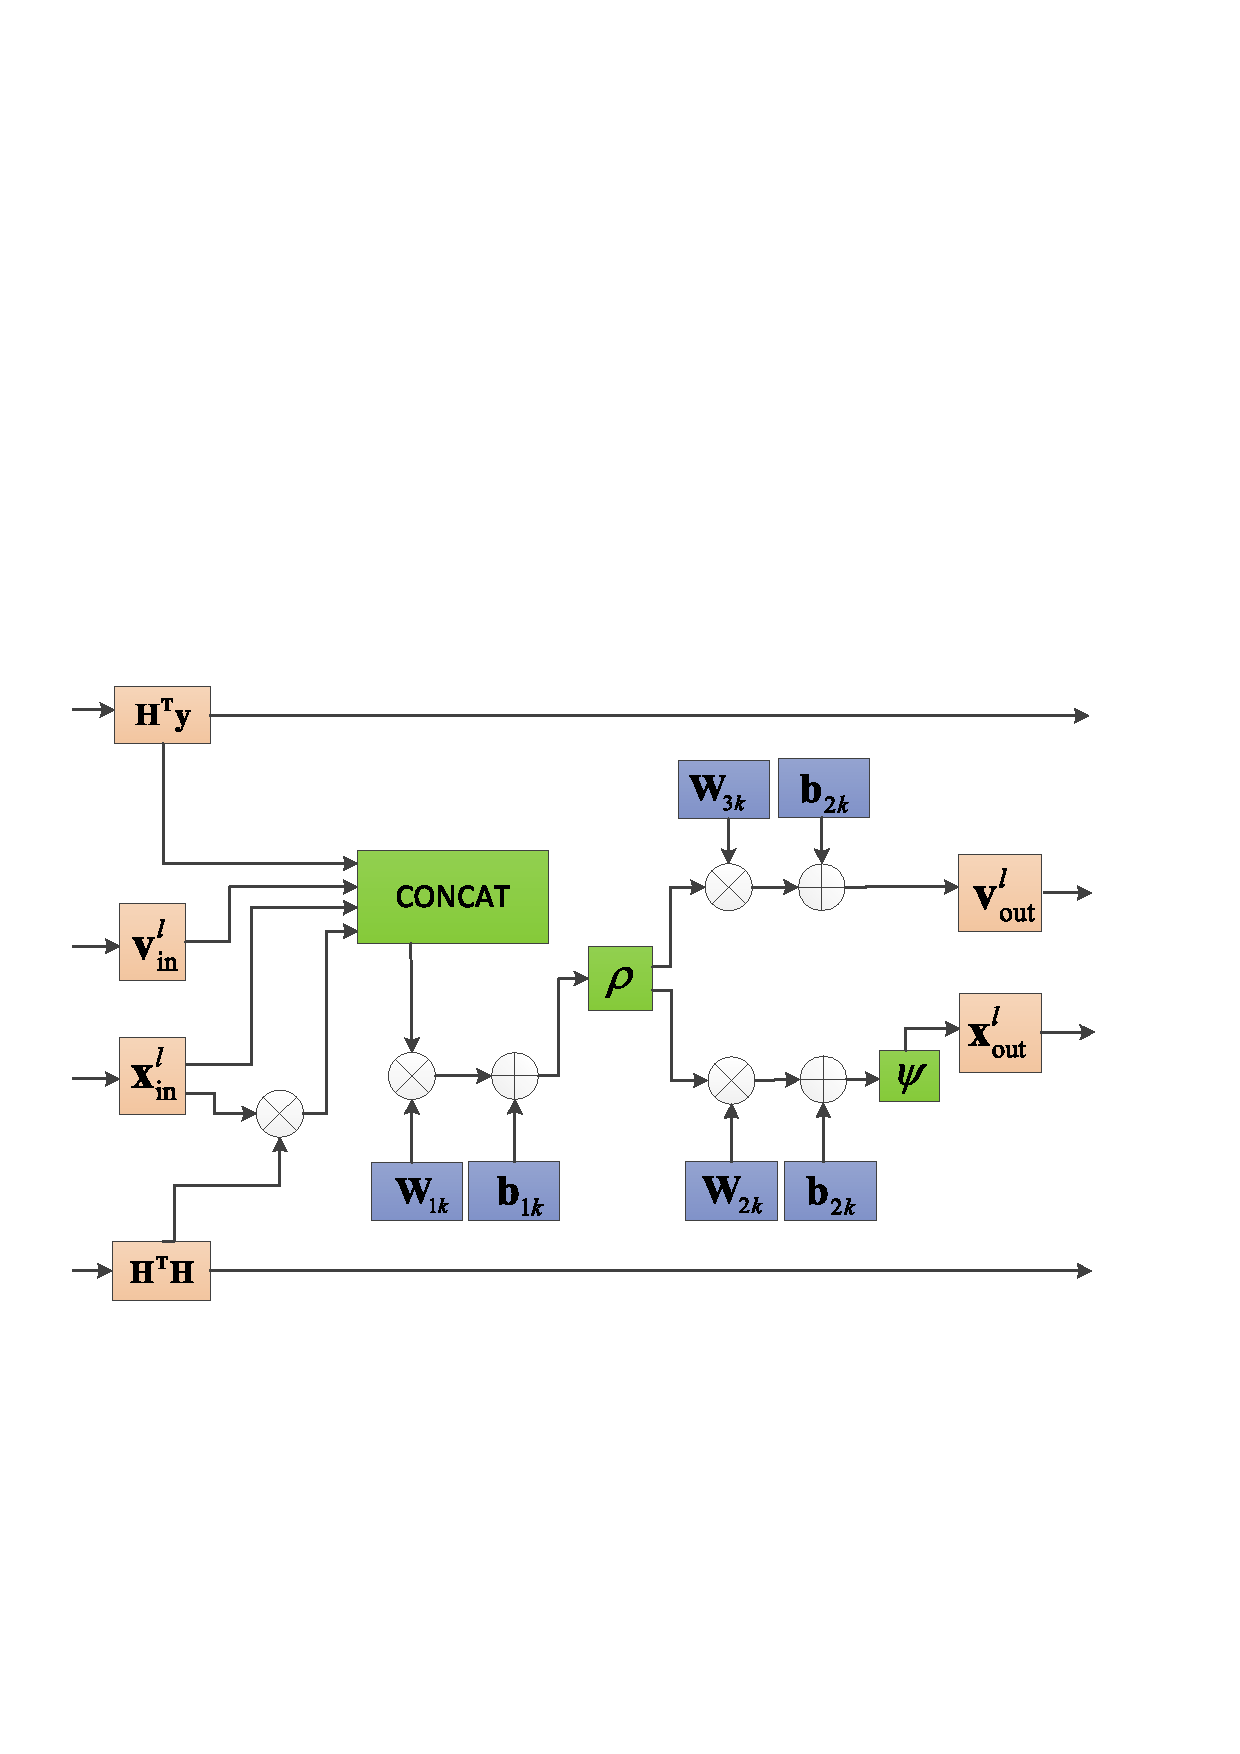
\includegraphics[width=0.5\textwidth]{DetNet.pdf}
%   \caption{Network Structure of Each Unit}
%   \label{DetNet unit}
% \end{figure}


\begin{table}[!htbp]
\centering
\caption{Network Structure of Each Unit}
\label{unit}
\begin{tabular}{|c|c|c|c|}
\hline
input & CONCAT & hidelayer  & output \\
\hline
${\textbf{H}^{T}\textbf{y}}$ & \multirow{4}{*}{${5n \times 1}$} & \multirow{4}{*}{${13n \times 1}$} & \multirow{2}{*}{${\textbf{v}_\textrm{out}^l }$}  \\

\cline{1-1} ${\textbf{v}_{\textrm{in}}^l}$ & & & \\
\cline{1-1} \cline{4-4} ${\textbf{x}_\textrm{in}^l}$ & & &\multirow{2}{*}{${\textbf{x}_\textrm{out}^l }$} \\
\cline{1-1} ${\textbf{H}^{T}\textbf{H}\textbf{x}}$ & & & \\
\hline
\end{tabular}
\end{table}

The dimension of ${\textbf{H}^T\textbf{y}}$ is ${n \times 1}$, the dimension of \textbf{v} is ${2n \times 1}$, the dimension of \textbf{x} is ${n \times 1}$, the dimension of ${\textbf{H}^T\textbf{H}}$ is ${n \times n}$. CONCAT is used to connect all the input vectors and transform them into a one-dimensional vector, the dimension of the output vector from CONCAT is ${5n \times 1}$. Then the output is transmitted through a full-connected network with a large number of nodes to map the output to a higher dimension. $\rho$ is sigmod function as activation function. Because each unit needs to be iterated, the final output of each unit should have the same dimension as the input \textbf{x} and \textbf{v}. So the output of $\rho$ is as the input to a layer of network for being compresssed to \textbf{v} and \textbf{x} dimensions. Since the final \textbf{x}${\in\{\pm1\}^K}$, the activation function used is similar to function $tanh$ whose range is (-1,1).

The loss function of the network is as follows:

\begin{equation}
\label{lossFunction}
Loss=\sum_{l=1}^L\log\left(l\right)\frac{\|\textbf{x}-\hat{\textbf{x}}_l\|^2}{\|\textbf{x}-\widetilde{\textbf{x}}\|^2}
\end{equation}
where:
\begin{equation*}
\label{lossFunction}
\widetilde{\textbf{x}}=\left(\textbf{H}^T\textbf{H}\right)^{-1}\textbf{H}^T\textbf{y}
\end{equation*}
$L$ is the total number of units. ${\hat{\textbf{x}}_l}$ is the unit $l$'s estimate of the transmitted vector.



\section{Improved DetNet}

Although DetNet is a good-performance MIMO detection neural network model, we still find there is room for improvements. In this section, we simplify the network. The simplifed network is a sparsely connected neural network called ScNet.

We take ${2 \times 2}$ MIMO structure as an example, and expand the network in Fig.\ref{DetNet unit} into the form of nodes, as in Fig.\ref{DetNetConnect}. Each node in Fig.\ref{DetNetConnect} represents one of the elements of vector.
\begin{figure}[ht]
  \centering
  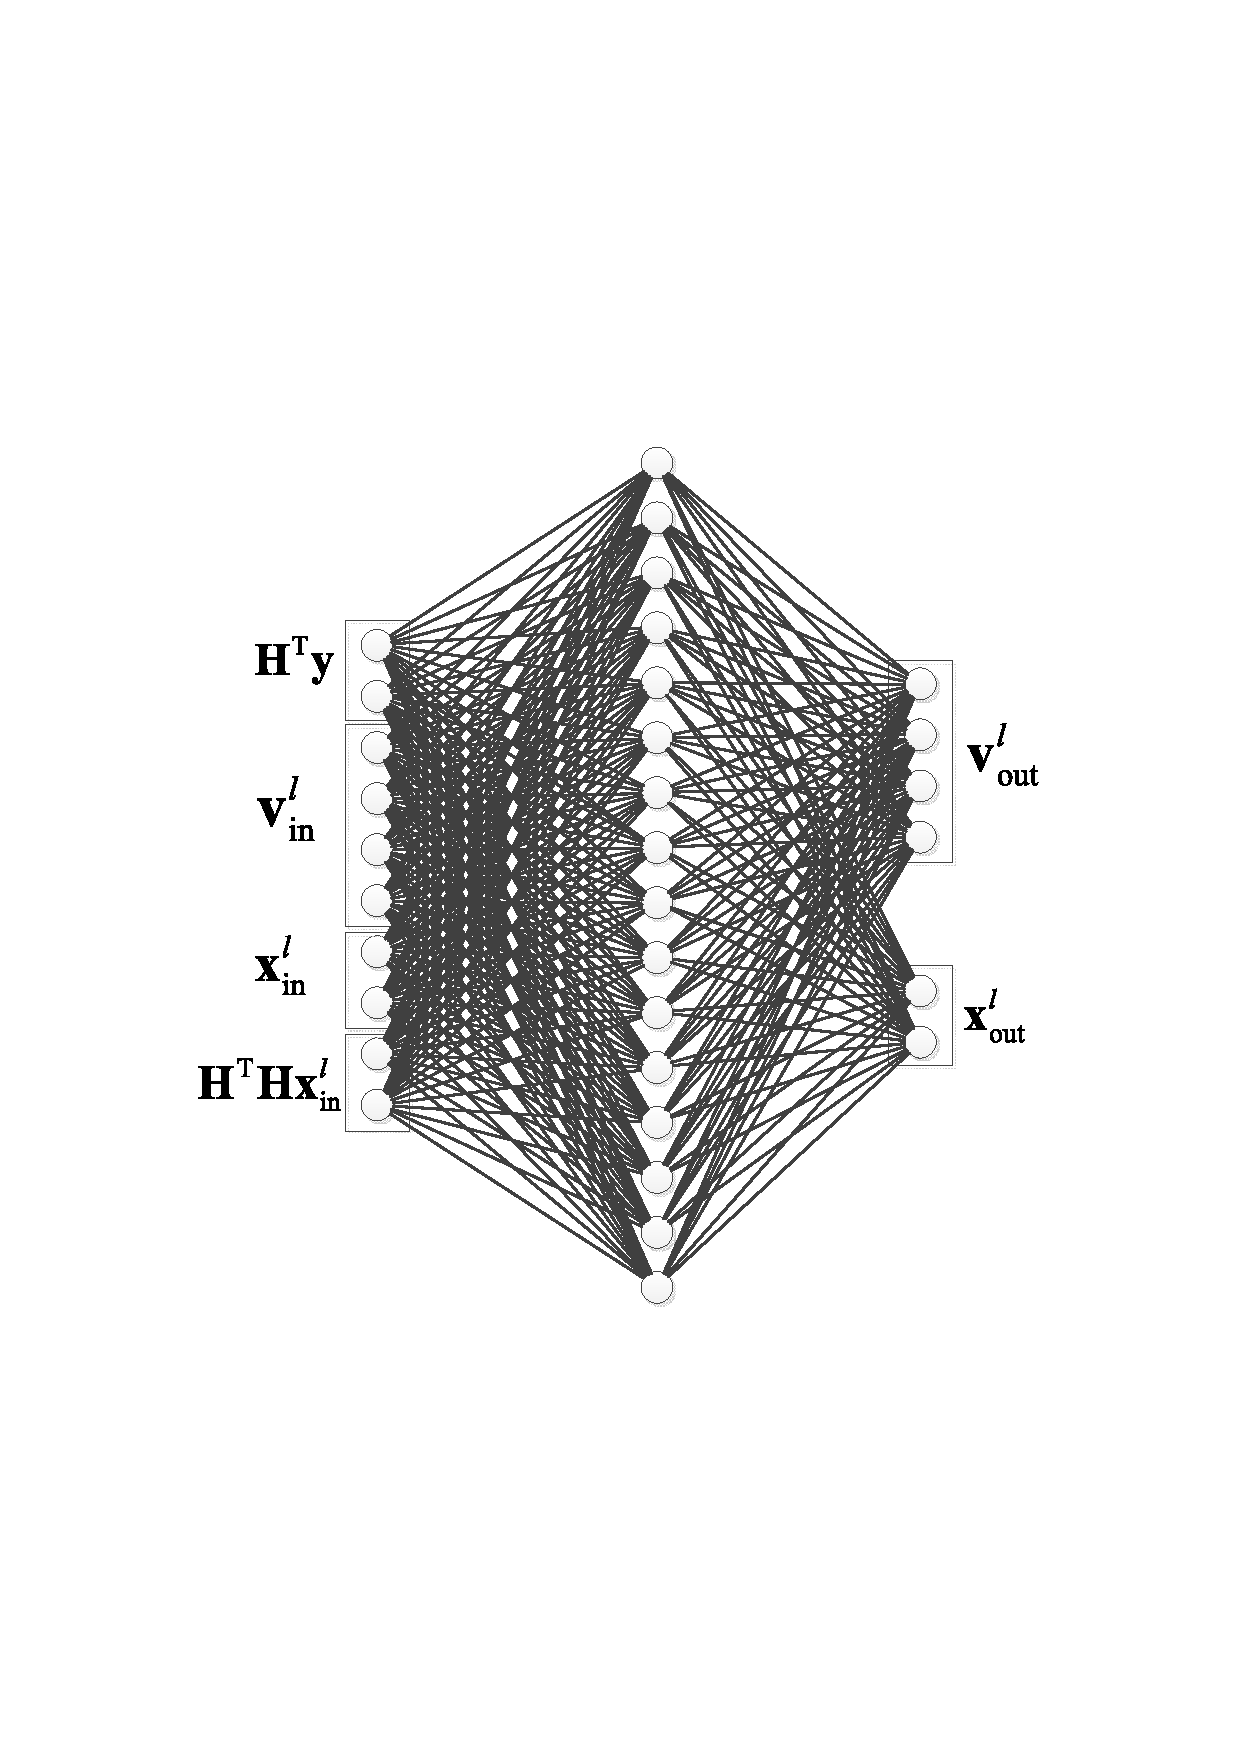
\includegraphics[width=0.4\textwidth]{DetNetConnect.pdf}
  \caption{DetNet Network Connection}
  \label{DetNetConnect}
\end{figure}

Our improvement includes three aspects, next we will elaborate on these three aspects in detail.

\subsection{Input Simplification} In Fig.\ref{DetNetConnect}, although there are two outputs: \textbf{x} and \textbf{v}, only one output is used as the approximation of the transmitted signal \textbf{x}. The other output \textbf{v} does not carry any information, just as the input/output filling, its role is similar to the role of network bias. By adding \textbf{v}, each unit increases a large number of connections and the complexity of the network. For the entire network, \textrm{v} has no physical meaning in the field of communications, and the removal of \textbf{v} simplify the network structure remarkably. With \textbf{v}, the number of edges per unit is ${8n \times 8n}$, and without \textbf{v}, the number of edges \textbf{v} is ${4n \times 8n}$. The total number of connections is reduced by half and the training parameters are reduced by half. After removing \textbf{v}, the network is shown in Fig.\ref{DetNetRemoveV}.

\begin{figure}[ht]
  \centering
  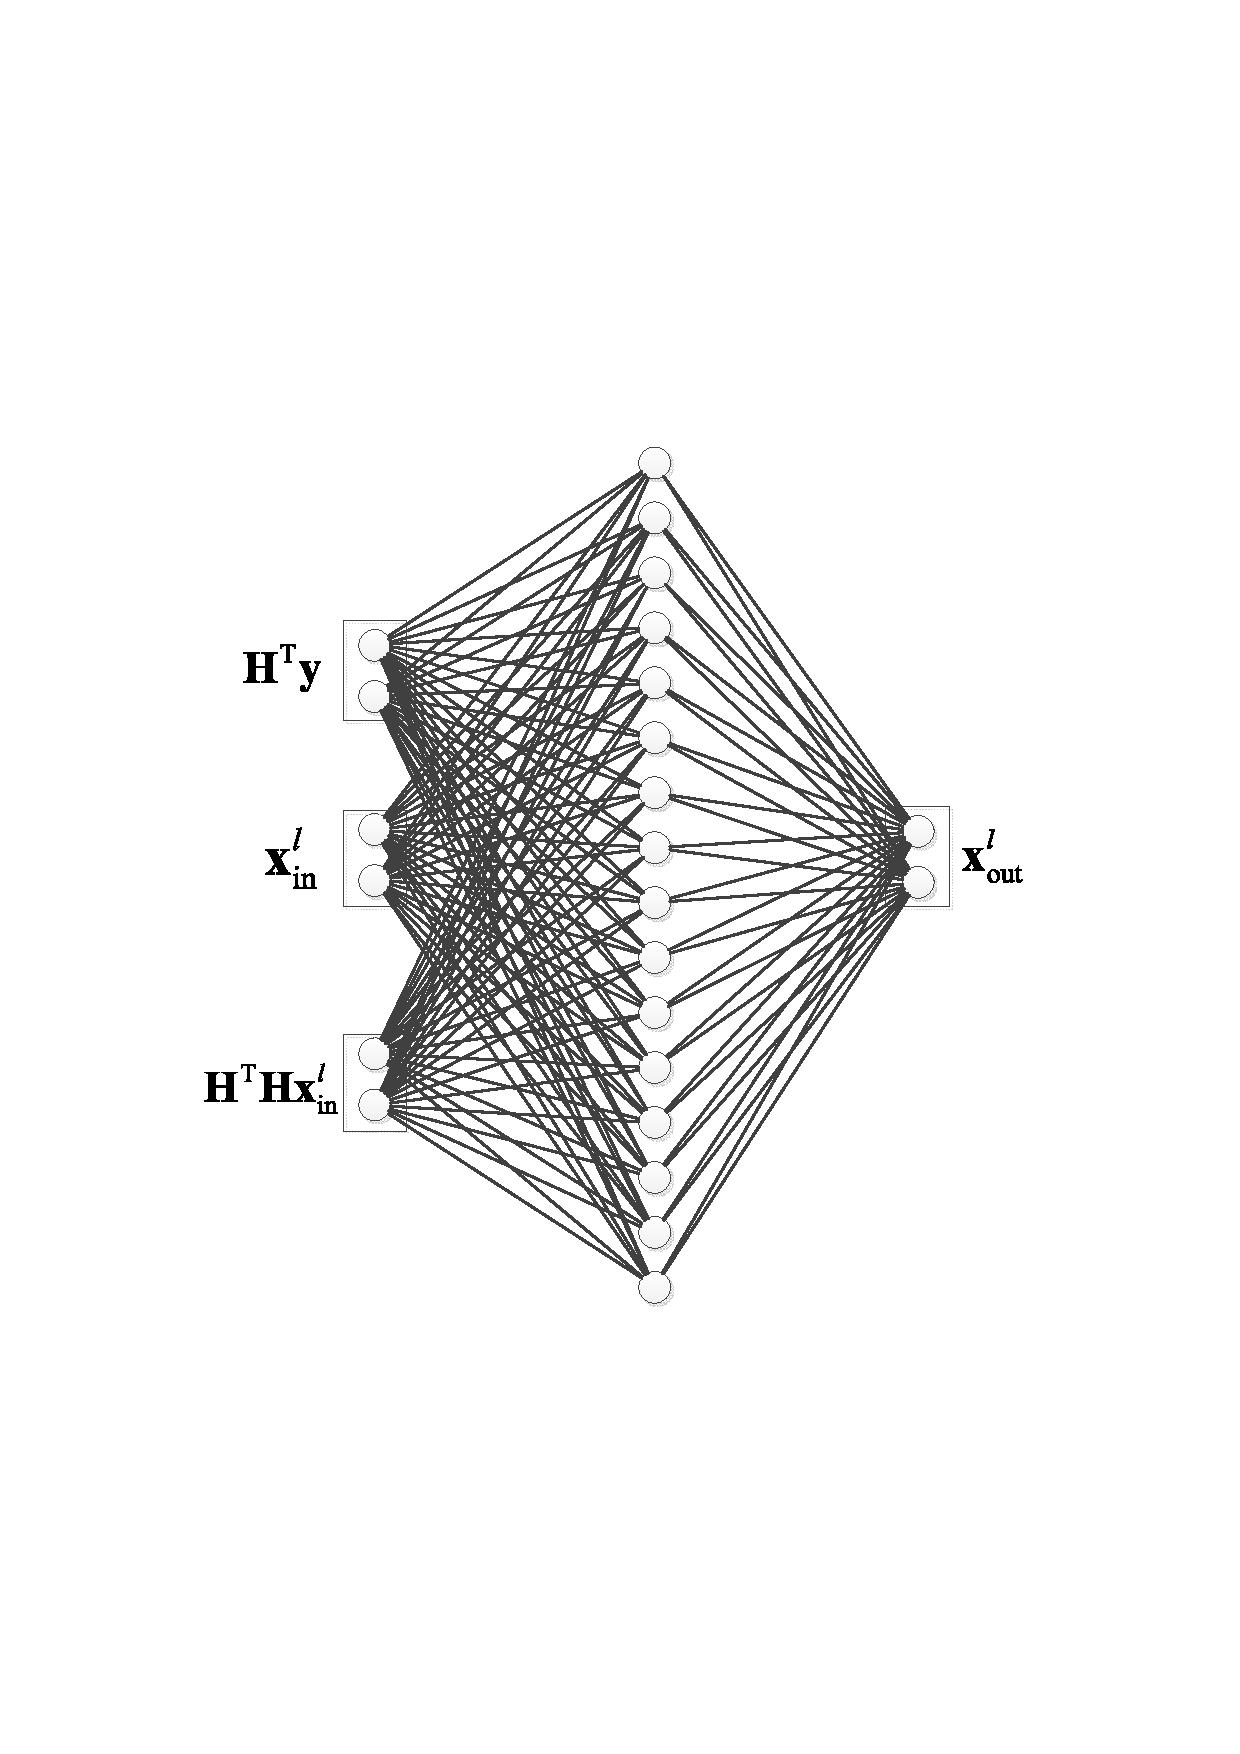
\includegraphics[width=0.4\textwidth]{DetNetRemoveV.pdf}
  \caption{DetNet Network Remove \textbf{v}}
  \label{DetNetRemoveV}
\end{figure}

It tested the network after removing \textbf{v} and find that the performance has small gain, and the training time is reduced.

\subsection{The Simplification of the Network Connection} After removing \textbf{v}, the network units are still fully connected structure. For each input node, it interacts with other nodes, but from formula (\ref{DetNetTheory}), the iterative structure describes linear operation of vectors. As shown in Fig.\ref{vector}, only the same indexed elements are added or subtracted in linear operation. Inspired by this mathematical principle, we connect the same indexed vector in the network to the output. The connection relationship is as Fig.\ref{ScNet}.

\begin{figure}[ht]
  \centering
  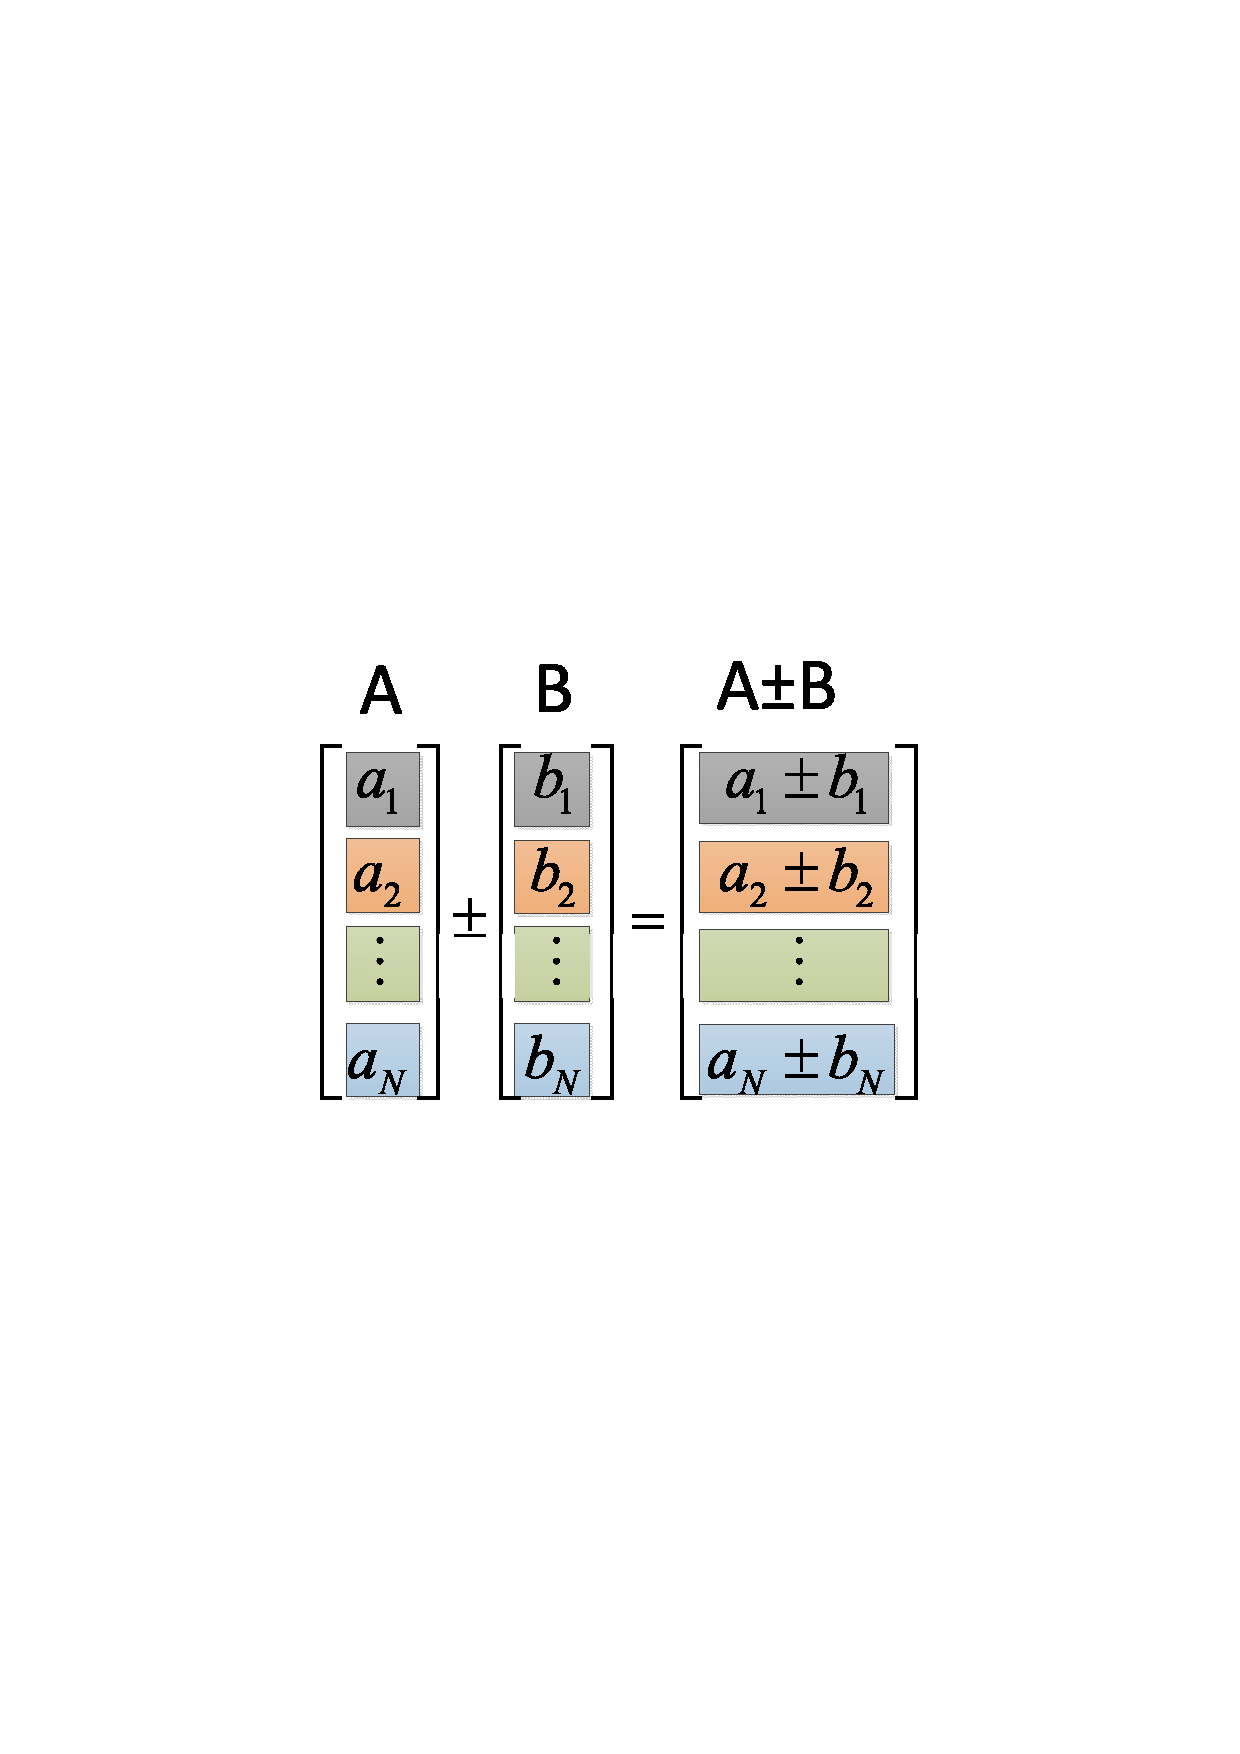
\includegraphics[width=0.3\textwidth]{vectorPlus.pdf}
  \caption{Vector Plus Vector}
  \label{vector}
\end{figure}

% 描述信息节点之间的交互关系
It is a sparsely connected neural network(ScNet). In ScNet, the first node of each input is only connected with the first node of output, the second node only connected with the second node of output. Regard node ${\textbf{x}_{\textrm{out}}^{l}[i]}$ of Fig.\ref{ScNet} as a medium of information exchange between ${\textbf{H}^T\textbf{y}[i]}$, ${\textbf{x}_{\textrm{in}}^l[i]}$ and ${\textbf{H}^T\textbf{Hx}_{\textrm{in}}^l[i]}$. $i$ denotes the index.

\begin{figure}[ht]
  \centering
  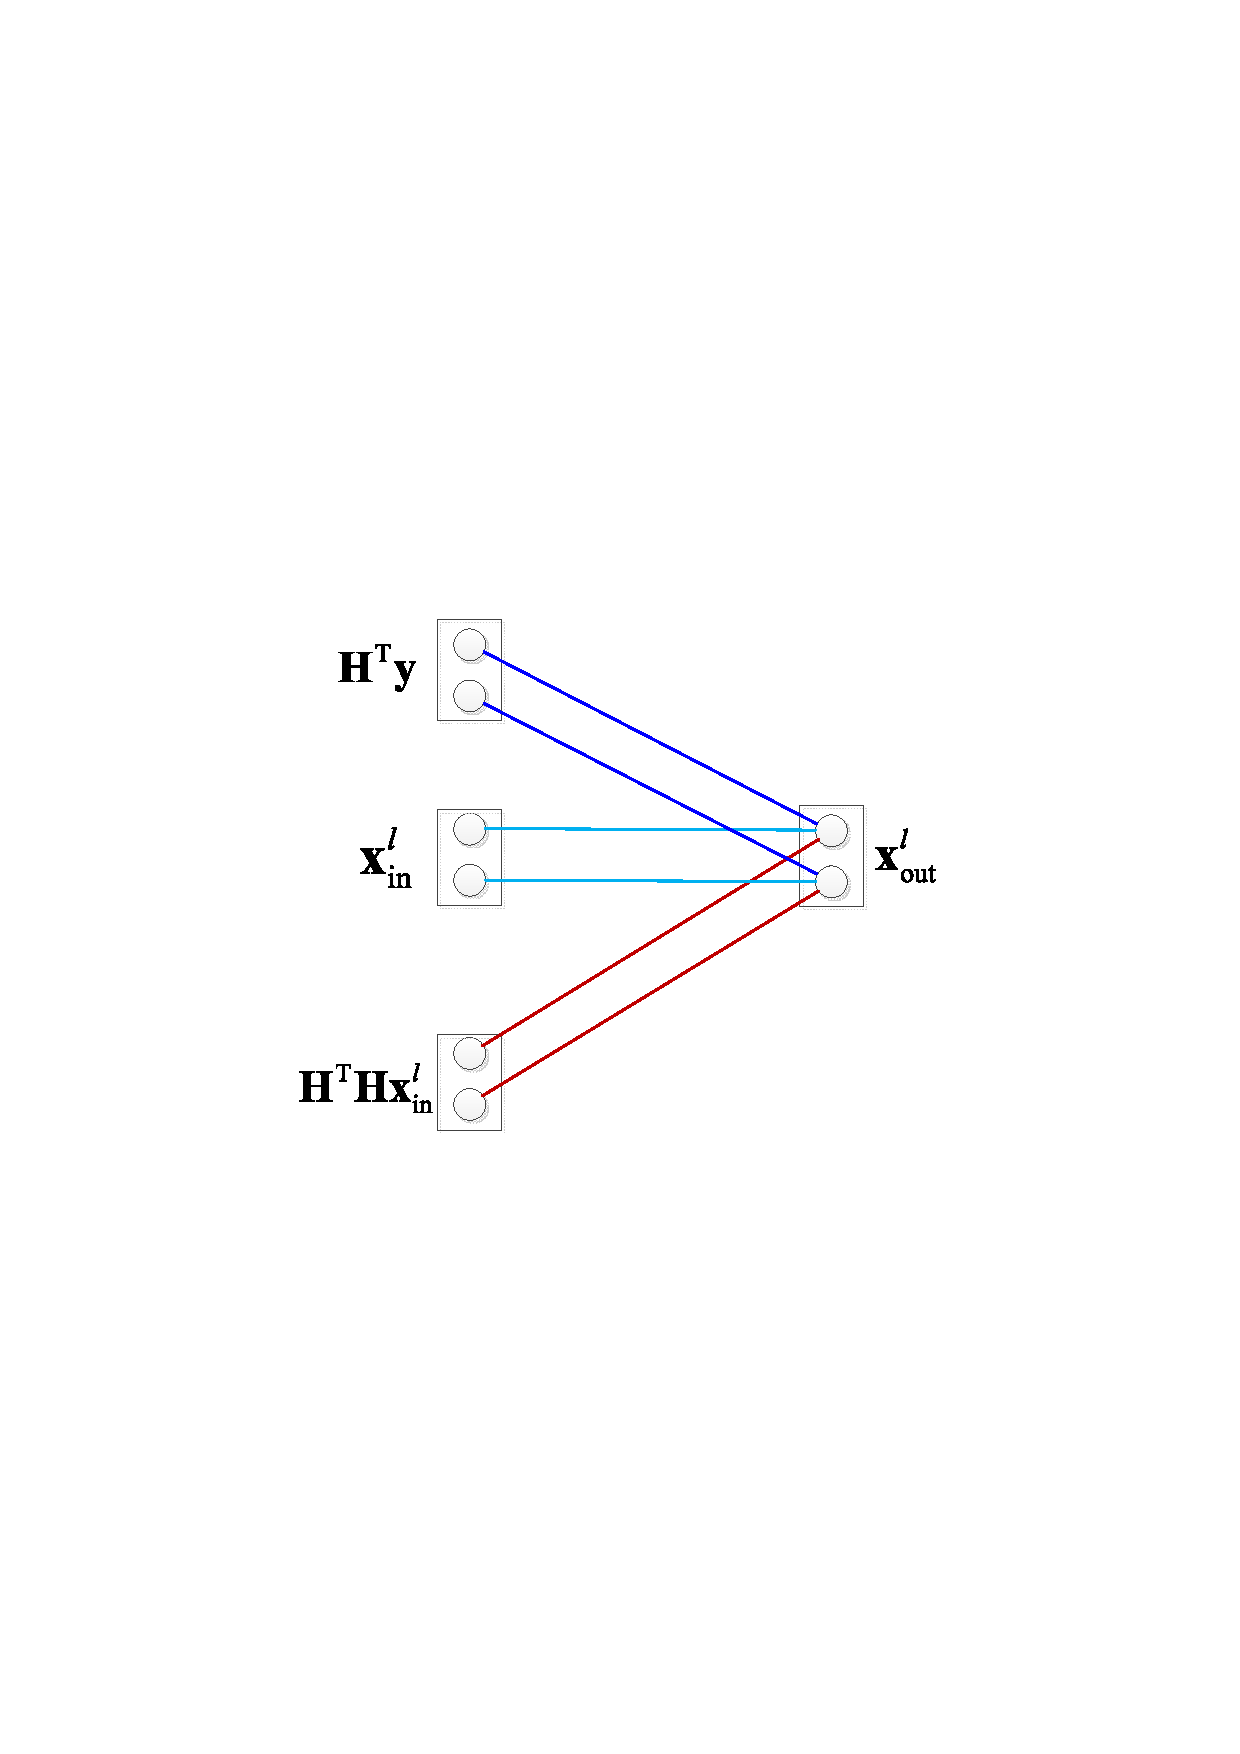
\includegraphics[width=0.3\textwidth]{ScNet.pdf}
  \caption{neural network connection for ScNet}
  \label{ScNet}
\end{figure}

Before simplification, the number of edges of each unit is ${8n \times 8n}$. After removing \textbf{v} and simplifying the network connection, the number of connected edges of the network is only ${3n}$.


\subsection{The Simplification of the Loss Function} The loss function for ScNet is as formula (\ref{ScNetLoss}):

\begin{equation}
\label{ScNetLoss}
Loss=\sum_{l=1}^L\log\left(l\right)\|\textbf{x}-\hat{\textbf{x}}_l\|^2
\end{equation}
Our loss function removes ${\|\textbf{x}-\left(\textbf{H}^T\textbf{H}\right)^{-1}\textbf{H}^T\textbf{y}\|^2}$ compared to DetNet's loss function. Actually the removal formula is equivalent to ${\|\textbf{n}\|^2}$. Our goal is to make Euclidean distance between estimations Euclidean distance of the output and send signals as close as possible, that isn't related to ${\|\textbf{x}-\left(\textbf{H}^T\textbf{H}\right)^{-1}\textbf{H}^T\textbf{y}\|^2}$, therefore, we remove the formula. Another reason that we remove this formula is: this formula contains matrix inversion operation, in many cases, the square matrix is not reversible and matrix inversion is a very complicated calculation. After our tests we find that after this formula is removed, the performance is improved slightly.

In our simulation, after the output of the last layer passes through the $\Psi$ activation function, the range will be ${\textbf{y}\in\left(-1,1\right)}$, we judge the results by (\ref{outjudge}).
\begin{equation}
\label{outjudge}
\textbf{y}_{\textrm{out}}=\left\{
\begin{aligned}
&1  &\mbox{${\textbf{y}_{\textrm{out}}^N\geqslant0}$}\\
&0  &\mbox{${\textbf{y}_{\textrm{out}}^N<0}$}
\end{aligned}
\right.
\end{equation}

In this section, inspired by DetNet, we propose a simplified deep learning model for MIMO detection called ScNet. In the following sections, we will compare the performance of these two networks.

\section{Simulation Results}

In this section, we compared the performance of DetNet and ScNet, the simulation conditions are as follows: all simulation channels is given fast fading channels, and the SNR of each simulation is randomly chosen in the range of [7, 14].
\begin{figure}[ht]
  \centering
  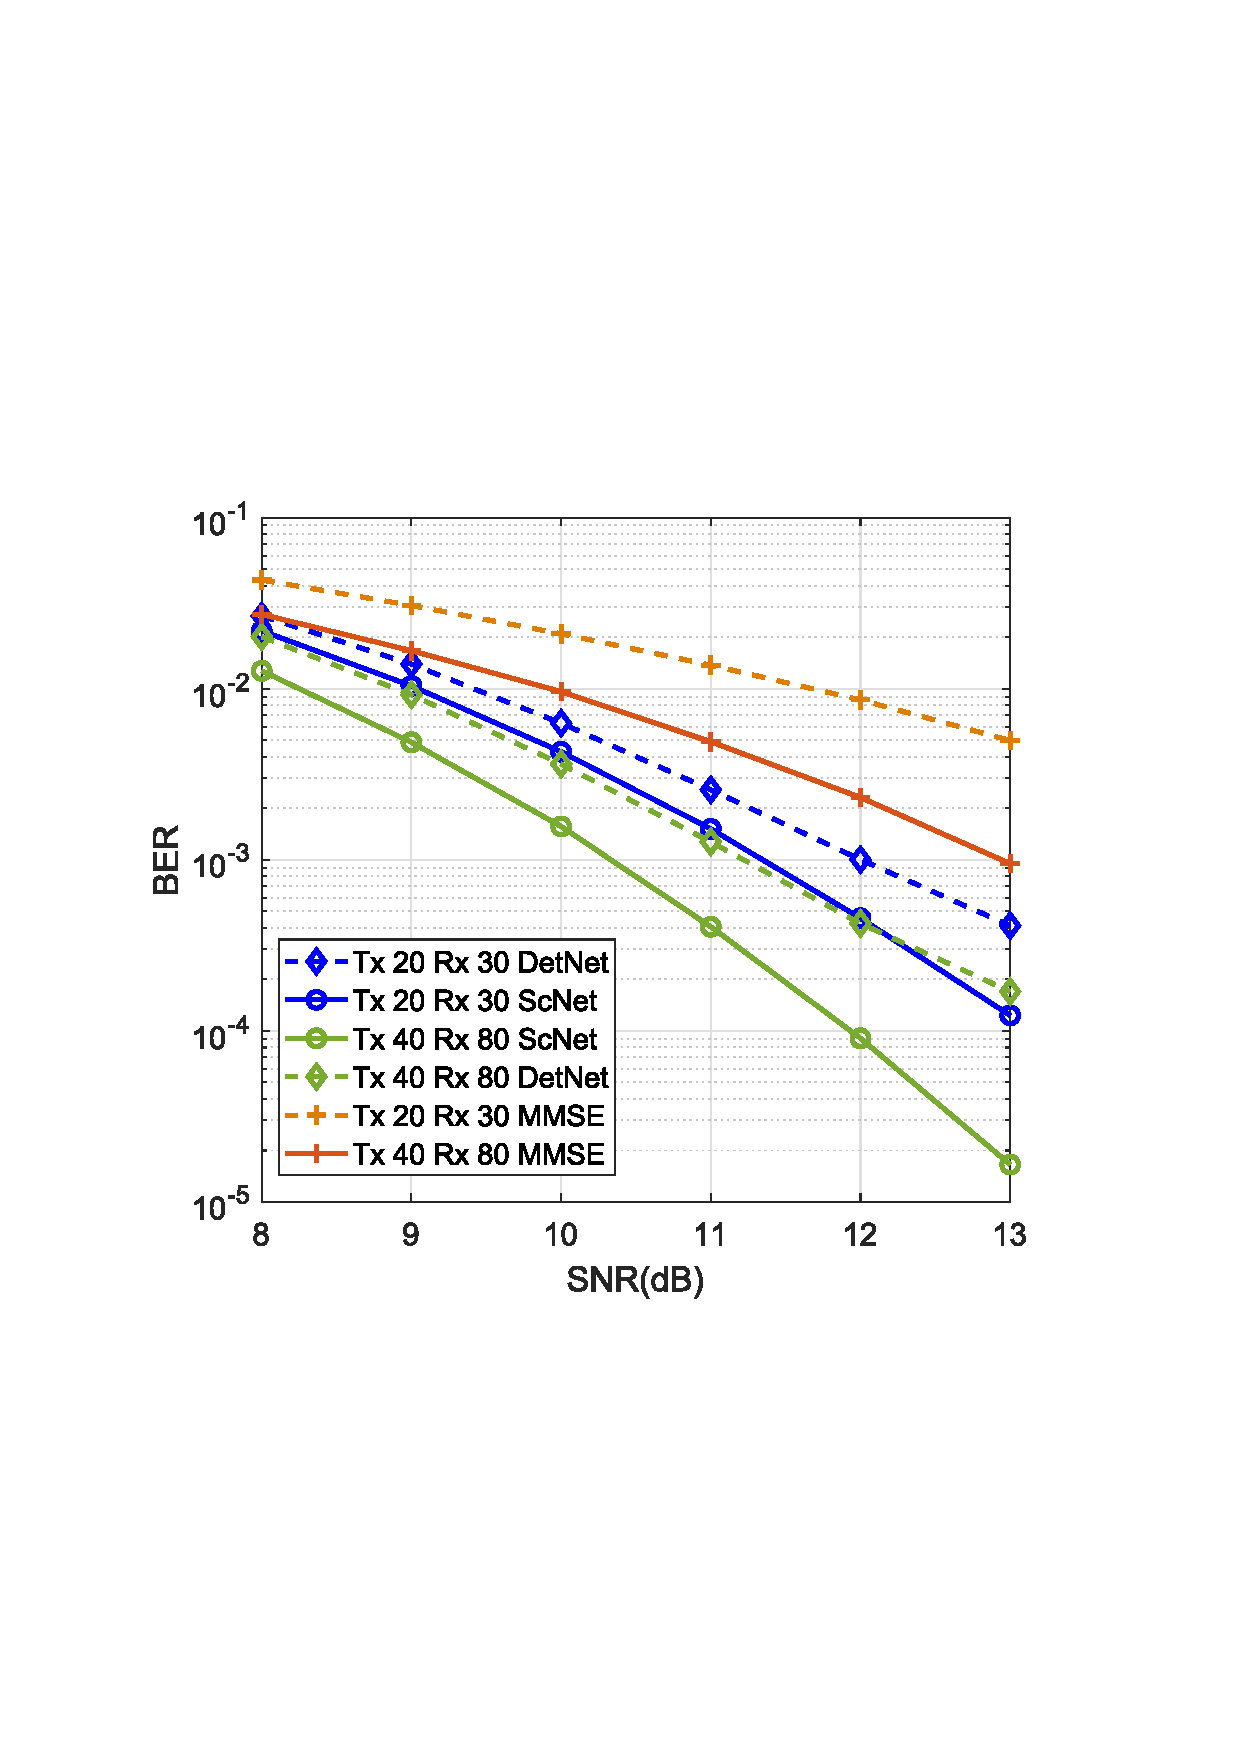
\includegraphics[width=0.48\textwidth]{Figcompare1.pdf}
  \caption{Comparing the Performance of DetNet and ScNet}
  \label{PerformanceCompare}
\end{figure}
At the beginning, the input \textbf{x} and \textbf{v} are into zero vectors. In DetNet, the dimension of \textbf{v} is ${2 \times n}$, the extended dimension from inputs is ${8 \times n}$ and the learning rate is 0.0001. The layer number of the two networks is 90 and the residual coefficient of the residual network choose 0.9. During training, we send ${5000 \times n}$ bits per antenna, which is recorded as one iteration. Table.\ref{edgesCompare} is the comparison of DetNet and ScNet, that is a reference to the complexity of the network.


\begin{table}[!htbp]
\centering
\caption{The comparison of Network Unit edge number}
\begin{tabular}{|c|c|c|} %表格7列 全部居中显示
\hline
antennas&network&unit edges \\
\hline
\multirow{2}{*}{Tx 20 Rx 30} & DetNet & 25,600 \\
\cline{2-3} &ScNet & 60 \\
\hline
\multirow{2}{*}{Tx 40 Rx 80} & DetNet & 102,400 \\
\cline{2-3} &ScNet & 120 \\
\hline
\end{tabular}
\label{edgesCompare}
\end{table}

Fig.\ref{PerformanceCompare} is a performance diagram comparing the two nets, it contains simulation results for two antenna configurations, Tx 20, Rx 30 and Tx 40, Rx 80. It can be seen that with Tx 40, Rx 80, the performance gain of ScNet over DetNet is about 1dB at ${10^{-4}}$.  Regardless of the antenna configuration, the performance of ScNet is slightly improved compared with DetNet, and far exceeds the performance of MMSE. Compared with the two antenna configurations of the same network, it can be seen that when the number of antennas increases, the performance gains. This shows that the ScNet with deep learning is more suitable for scenarios with large scale of antennas.

\begin{figure}[ht]
  \centering
  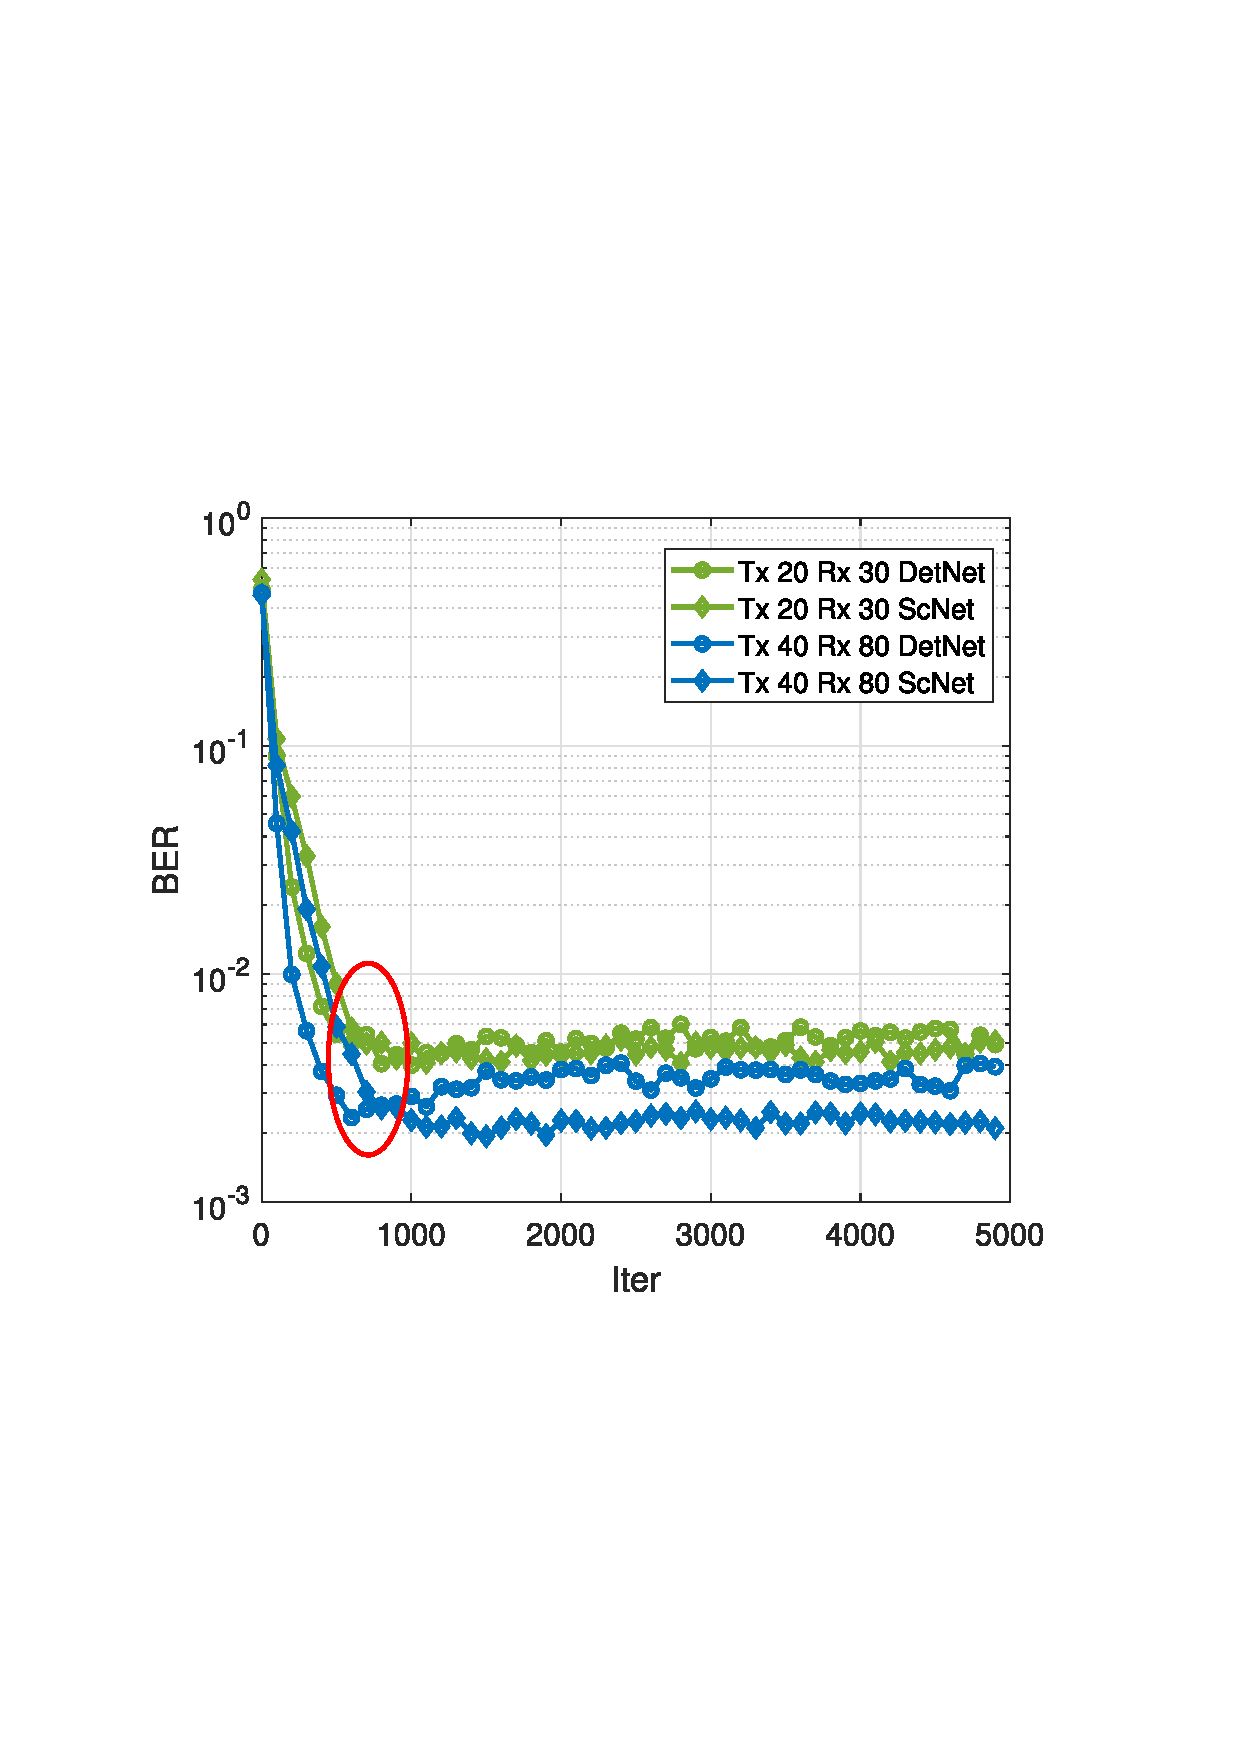
\includegraphics[width=0.48\textwidth]{convergence.pdf}
  \caption{Network Convergence Speed}
  \label{Convergence}
\end{figure}

Fig.\ref{Convergence} shows the convergence speeds of the two network trainings. The random SNR is used to test when these two networks are trained, so the BER after convergence does not reach the minimum value, and the network fluctuation is also slightly larger. It can be seen that, however, the simplification of the network has not affected the convergence performance of the network.

\section{Conclusions and Future Work}
In this paper, an improved deep learning model is proposed for detection in large-scale MIMOs, based on the analysis of DetNet model. Numerical analysis indicates that ScNet not only simplifies the complexity, but also improves the performance, especially when sending and receiving end equipped with large scale antenna.

\section*{Acknowledgment}
This work was supported by the National Natural Science Foundation of China (No. 61601047, 61671080, 61771066),  and Science and Technology on Communication Networks Laboratory Open Project (KX172600028).




\begin{thebibliography}{1}

\bibitem{LTE}
E. Dahlman, S. Parkvall, J. Sköld, P. Beming, "3G Evolution HSPA and LTE for Mobile Broadband". Academic, 2008.

\bibitem{MIMO1}
F. Rusek, D. Persson, B. K. Lau, E. G. Larsson, T. L. Marzetta,O. Edfors, and F. Tufvesson, "Scaling up mimo: Opportunities and challenges with very large arrays", \emph{IEEE Signal Processing Magazine}, vol. 30, no. 1, pp. 40~C60, 2013.

\bibitem{MIMO2}
S. Yang and L. Hanzo, "Fifty years of mimo detection: The road to large-scale mimos",\emph{IEEE Communications Surveys \& Tutorials}, vol. 17, no. 4, pp. 1941~1988, 2015.

\bibitem{AMP}
S. Wu, L. Kuang, Z. Ni, J. Lu, D. Huang and Q. Guo, "Low-Complexity Iterative Detection for Large-Scale Multiuser MIMO-OFDM Systems Using Approximate Message Passing", in IEEE Journal of Selected Topics in Signal Processing, vol. 8, no. 5, pp. 902-915, Oct. 2014.

\bibitem{SDR}
Z. Ma, M. Zhao, Q. Chen and P. Fan, "MIMO detection for high-order QAM constellations based on successive decision feedback semidefinite relaxation," Proceedings of the Fifth International Workshop on Signal Design and Its Applications in Communications, Guilin, 2011, pp. 173-176.

\bibitem{detector}
J. Jalden and B. Ottersten, "The diversity order of the semidefinite relaxation detector", \emph{IEEE Transactions on Information Theory}, vol. 54, no. 4, pp. 1406~C1422, 2008.

\bibitem{FSD}
C. Xiong, X. Zhang, K. Wu and D. Yang, "A simplified fixed-complexity sphere decoder for V-BLAST systems", in IEEE Communications Letters, vol. 13, no. 8, pp. 582-584, August 2009.

\bibitem{XGBoost}
T. Chen and C. Guestrin. "Xgboost: A scalable tree boosting system". CoRR, abs/1603.02754, 2016.

\bibitem{normalization}
S. Ioffe and C. Szegedy. "Batch normalization: Accelerating deep network training by reducing internal covariate shift". arXiv:1502.03167, 2015

% \bibitem{sum-product}
% F. R. Kschischang, B. J. Frey and H. A. Loeliger, "Factor graphs and the sum-product algorithm", in IEEE Transactions on Information Theory, vol. 47, no. 2, pp. 498-519, Feb 2001.

\bibitem{ResNet}
K. He X. Zhang S. Ren J. Sun "Deep Residual Learning for Image Recognition", in \emph{Computer Vision and Pattern Recognition IEEE} pp. 770-778 2016.


\bibitem{DetNet}
N. Samuel, T. Diskin and A. Wiesel, "Deep MIMO detection" \emph{2017 IEEE 18th International Workshop on Signal Processing Advances in Wireless Communications (SPAWC)}, Sapporo, 2017, pp. 1-5. doi: 10.1109/SPAWC.2017.8227772






\end{thebibliography}




% that's all folks
\end{document}


